%%%%%%%%%%%%%%%%%%%%%%%%%%%%%%%%%%%%%%%%%%%%%%%%%%%%%%%%%%%%%%%%%%%%%%
%%                     Equivalence Arc
%%%%%%%%%%%%%%%%%%%%%%%%%%%%%%%%%%%%%%%%%%%%%%%%%%%%%%%%%%%%%%%%%%%%%%

\subsection{Glyph: \glyph{Equivalence arc} }\label{sec:equivalenceArc}

\glyph{Equivalence Arc} is the arc used to represent the fact that all activities or compartments
marked by a \glyph{tag} are equivalent.

\begin{glyphDescription}
 \glyphSboTerm Not applicable.
 \glyphOrigin Any \glyph{Activity node} (\sect{af:ANs}) or any \glyph{compartment}.
 \glyphTarget \glyph{Tag}.
 \glyphEndPoint No particular symbol is used to represent an \glyph{equivalence arc}.
 \end{glyphDescription}

\begin{figure}[H]
  \centering
  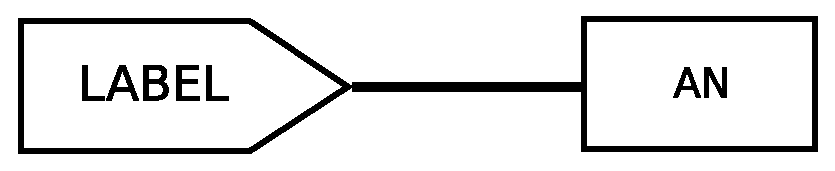
\includegraphics[scale = 0.4]{images/equivalence}
  \caption{The \AF glyph for \glyph{Equivalence arc}.}
  \label{fig:equivalence}
\end{figure}
